\section{Multivariable control}
\subsection{Introduction}
As the helicopter is a complex system with multiple states, it is reasonable to implement a multivariable control system.
The system is controlled by an LQR-controller, as it provides an intuitive way to design a control rule based on minimizing a cost function. 
Analyzing the controllability matrix of the system showed that the system was indeed controllable.
Because the LQR controller provides the feedback gain maktrix $K$ which minimizes a cost function based on the states and input, it will naturally try to drive the states towards 0. 
In order to actually have the states reach their target reference, a feed forward input is also implemented. 
Lastly because our system, and also thus our control rules, are based on a linearized approximation of the real system there has been added an integral action to remove the steady-state error.

The system matrices (before the integral action) are shown in \ref{eq:lab2-system1}.
\begin{equation}
\label{eq:lab2-system1}
   A = \begin{bmatrix}
	0 & 1 & 0 \\
	0 & 0 & 0 \\
	0 & 0 & 0
   \end{bmatrix},\; 
   B = \begin{bmatrix}
	0 & 0 \\
	0 & K_1 \\
	K_2 & 0
   \end{bmatrix}
\end{equation}
Using this we can calculate the controllability matrix \ref{eq:lab2-controllability}, which has a rank of 3 and the system is thus controllable. 
\begin{equation}
\label{eq:lab2-controllability}
   \mathcal{C} = \begin{bmatrix}
	0 & 0 & K_1 & 0 & 0 \\
	0 & K_1 & 0 & 0 & 0 \\
	K_2 & 0 & 0 & 0 & 0
   \end{bmatrix}
\end{equation}
Our control rule is then given by \ref{eq:lab2-control-rule}, where $K$ is given by LQR and $F$ is derived in \ref{eq:lab2-F} from $K$ to drive the system to our target reference $r$.
\begin{equation}
\label{eq:lab2-control-rule}
   u = -Kx + Fr
\end{equation}
\begin{equation}
\label{eq:lab2-F}
   F = \begin{bmatrix}
	K_{11} & K_{13} \\
	K_{21} & K_{23}
   \end{bmatrix}
\end{equation}
The system matrices (after the integral action) are shown in \ref{eq:lab2-system2}. 
The G matrix here is being multiplied the the reference.
\begin{equation}
\label{eq:lab2-system2}
	A = \begin{bmatrix}
		0 & 1 & 0 & 0 & 0 \\
		0 & 0 & 0 & 0 & 0 \\
		0 & 0 & 0 & 0 & 0 \\
		-1 & 0 & 0 & 0 & 0 \\
		0 & 0 & -1 & 0 & 0 
	\end{bmatrix},\;
	B = \begin{bmatrix}
		0 & 0 \\
		0 & K_1 \\
		K_2 & 0 \\ 
		0 & 0 \\ 
		0 & 0
	\end{bmatrix},\; 
	G = \begin{bmatrix}
		0 & 0 \\
		0 & 0 \\
		0 & 0 \\
		1 & 0 \\ 
		0 & 1
	\end{bmatrix}
\end{equation}

\subsection{Hypothesis and test plan}
All our test were conducted the same way with a test plan structured as this: 
\begin{itemize}
	\item Start up the system.
	\item Apply a change in the reference from 0 to $\frac{\pi}{4}$ between time 3s and 5s. 
	\item Simulate a disturbance by applying an external pulse in the input voltage at 13s.
\end{itemize}
The main things we wanted to test was how different choices of Q and R affected the sytem as well as how the integral action affected the system. 
We came up with 5 cases to test the relation between Q and R, and tested these 5 cases both with and without integral action:
\begin{itemize}
	\item $R = 5\mathbf{I},\; Q=\mathbf{I}$
	\item $R = 100\mathbf{I},\; Q=\mathbf{I}$
	\item $R = \mathbf{I},\; Q=5\mathbf{I}$
	\item $R = \mathbf{I},\; Q=100\mathbf{I}$
	\item $R = \mathbf{I},\; Q=\mathbf{I}$
\end{itemize}
Our Hypothesis were that an R larger than Q would give a slow system response as the cost of the input was weighted higher than the cost of the state, meanwhile the opposite would give a fast response. 
When both Q and R were equal to an identity matrix we hypothesized that we would get some form of balanced response. 
As for with or without integral gain our hypothesis was that the integral gain would remove the steady state error of the system.

\subsection{Results}
Here are the test results for all the cases
\subsubsection{$R = 5\mathbf{I},\; Q=\mathbf{I}$}
The pitch response fails to even respond to the reference at all without the integral action. The integral helps some but the response is still very sluggish.
\begin{figure}[H]
	\centering
	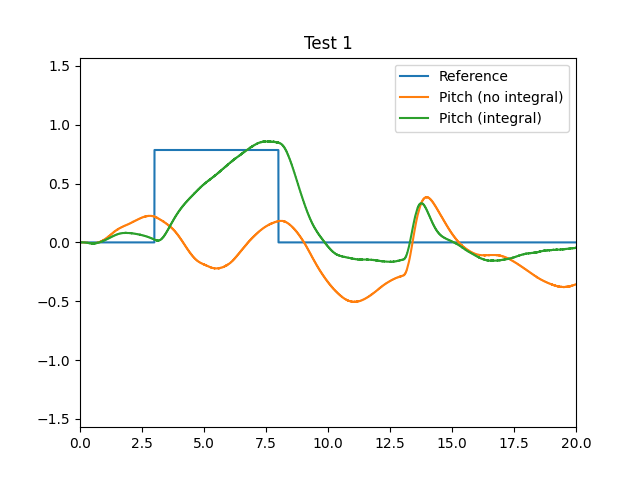
\includegraphics[width=0.6\textwidth]{figures/lab2-test1.png}
	\caption{Test result for test 1}
	\label{}
\end{figure}


\subsubsection{$R = 100\mathbf{I},\; Q=\mathbf{I}$}
As with the previous test, the response without integral fails to respond at all. THe integral helps some, but is way too slow to even reach the reference point.
\begin{figure}[H]
	\centering
	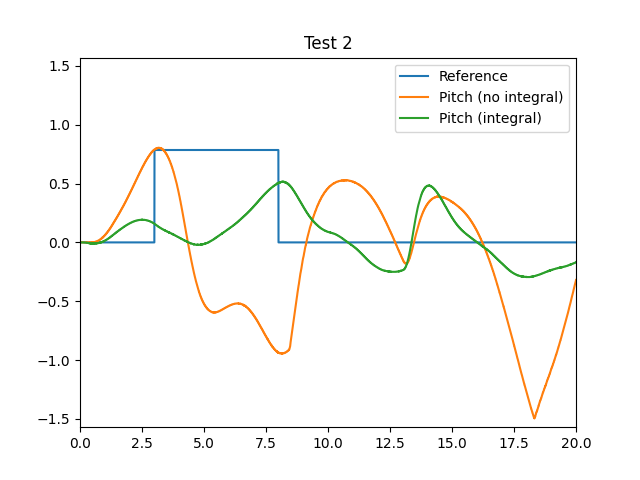
\includegraphics[width=0.6\textwidth]{figures/lab2-test2.png}
	\caption{Test result for test 2}
	\label{}
\end{figure}

\subsubsection{$R = \mathbf{I},\; 5Q=\mathbf{I}$}
Here the pitch is able to track the reference better, but does converge to a stationary error without the integral. The integral does overshoot a bit, but converges after to the reference. This can also be seen towards the end of the series. 
\begin{figure}[H]
	\centering
	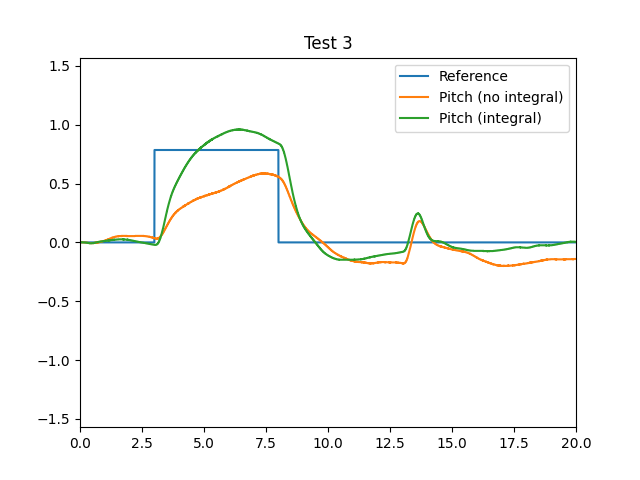
\includegraphics[width=0.6\textwidth]{figures/lab2-test3.png}
	\caption{Test result for test 3}
	\label{}
\end{figure}

\subsubsection{$R = \mathbf{I},\; 100Q=\mathbf{I}$}
The reference is being followed by both the controllers. The integral action eliminates the stationary error.
\begin{figure}[H]
	\centering
	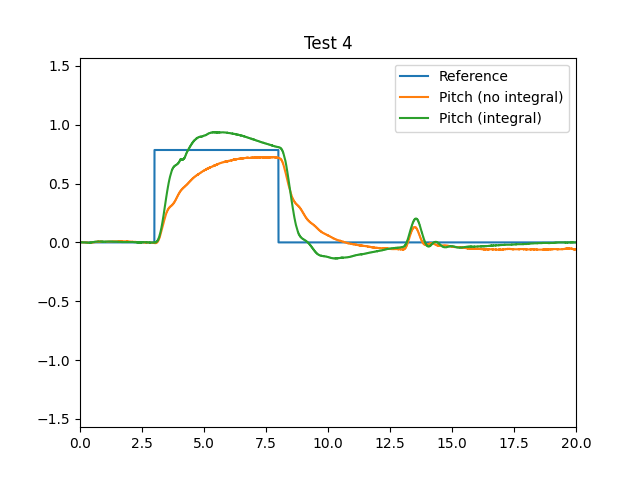
\includegraphics[width=0.6\textwidth]{figures/lab2-test4.png}
	\caption{Test result for test 4}
	\label{}
\end{figure}

\subsubsection{$R = \mathbf{I},\; Q=\mathbf{I}$}
Both signals track the reference, but both controllers are a bit slower to reach it. Also the controller with no integral action has a stationary error.
\begin{figure}[H]
	\centering
	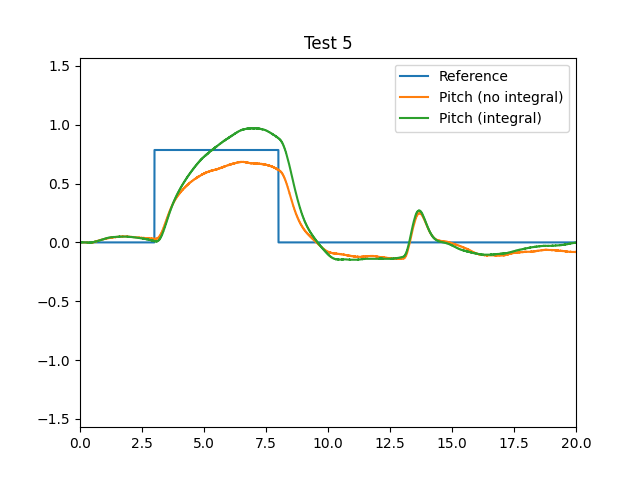
\includegraphics[width=0.6\textwidth]{figures/lab2-test5.png}
	\caption{Test result for test 5}
	\label{}
\end{figure}

\subsection{Conclusion}
All our hypotheses matched with our findings. The tests with high R and low Q had weak, in fact too weak, responses. The tests with high Q values and low R had very fast responses, while the test with equal Q and R values had converging but somewhat slow responses. In addition it was shown that the integral action helped remove the staionary error.